\documentclass[12pt]{scrartcl}
\usepackage{amsmath, amssymb, amsthm, mathtools}
\newtheorem{theorem}{Theorem}[section]
\newtheorem{corollary}{Corollary}[theorem]
\newtheorem{lemma}[theorem]{Lemma}

\usepackage{enumitem}
\usepackage{tikz, pgfplots}
\pgfplotsset{compat=1.17, width=10cm}
\usepgfplotslibrary{external}
\tikzexternalize

\usepackage{siunitx}

\usepackage[OT1]{fontenc}
\usepackage{mlmodern}
\usepackage{setspace}

\usepackage[backend=biber,style=numeric,sortcites=true]{biblatex}
\addbibresource{main.bib}
\usepackage{hyperref}

\title{The Bigger The Better II}
\author{Group 8-29 \thanks{Derrick Lukimin (L, 2i204), Tan Yong Yih (2i222), Wu Hao (2i324), Darren Yap (2i425)}}
\date{2022}

\begin{document}
\onehalfspacing
\maketitle
\tableofcontents

\section{Introduction}
This project aims to find an algorithm to determine
the side length of the largest square that can be
inscribed inside a convex $n$-gon. It is a continuation from
a previous project completed in 2021, The Bigger The Better. \cite{tbtb1}

\subsection{Definitions}
\begin{description}[font=\bfseries, leftmargin=1cm, style=nextline]
	\item[placement] A valid location, size and rotation of the square such that
		all vertices of the square lie on the edges of the polygon.
	\item[inscribed] All vertices of the square must lie on the edges of the polygon.
	\item[fit] All vertices of the square must lie within the polygon.
	\item[RQ] Research Question
\end{description}

\subsection{Research Questions}
\begin{enumerate}
	\item What is the side length of the largest square that can be inscribed in a triangle?
	\item What is the side length of the largest square that can be inscribed in a regular $n$-gon, given $n \neq 4$?
	\item What is the side length of the largest square that can be inscribed in a convex $n$-gon?
\end{enumerate}

\subsection{Project Scope}
This project will only focus on convex polygons.

\section{Literature Review}
\cite{tbtb1} gave a crucial insight into the investigation regarding RQ1 — that only three possible placements exist for the largest square within an acute triangle, each placement having one side of the square coinciding with each side of the triangle.
\cite{chazelle} gave insight and confirmation that fitting a square within a convex n-gon, in turn used for RQ2, was possible.
\cite{dilworth} allowed us to find an algorithm to check if a $n$-gon can be inscribed in a $m$-gon, given confirmation that doing so was possible.
\cite{emch} allowed us to prove that a square can always be inscribed inside a convex polygon, which helped us to formulate the ideas used in RQ3.

\pagebreak

\section{Research Question 1}

RQ1 aims to find out the side length of the largest square that can be inscribed in a triangle,
given the side lengths of the triangle, $a$, $b$ and $c$.

\subsection{Key Insights}
Some key insights which greatly aided in solving this problem were found.
\begin{enumerate}
	\item It can be seen that no more than two vertices of a square can lie on a single side,
	      as a square has at most two co-linear vertices.
	\item We notice how a triangle has three sides, and a square has four vertices.
	      In order for all the vertices to lie on the triangle, using the Pigeonhole Principle,
	      there will be at least one side with two vertices lying on it.
	\item Combining the above insights, there will be one vertex of the square
	      each lying on two sides of the triangle, with the other two vertices of the square
	      lying on the latter side of the triangle.
\end{enumerate}

\subsection{Solution}
A figure has been constructed for the purposes of illustrating the following proof.
\begin{figure}[htpb]
	\centering
	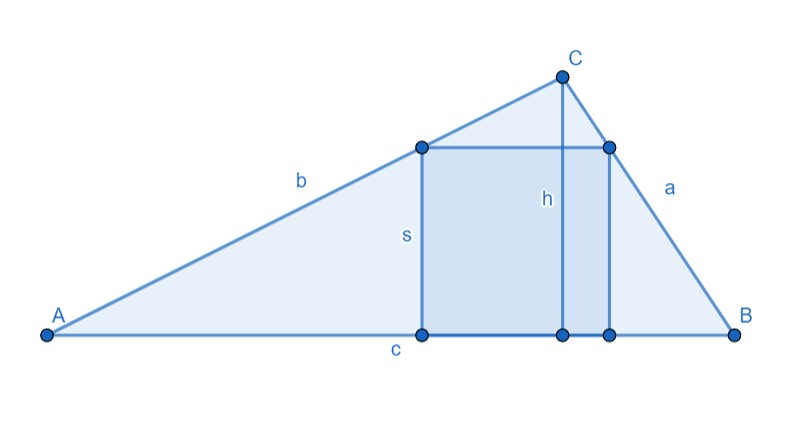
\includegraphics[scale=.75]{images/rq1.jpg}
	\label{fig:rq1_img}
	\caption{The figure for RQ1.}
\end{figure}

Let $s$ be the side length of the largest square that can be inscribed in a triangle,
with side lengths $a$, $b$ and $c$, and circumradius $R$.

Side $c$ can be formed with the sum of $s$, $s \cot A$ and $s \cot \angle{B}$.
Hence, we can express $s$ with the side length $c$, as well as angles $A$ and $B$.

\begin{align*}
	c & = s+s\cot \angle{A}+s\cot \angle{B}          \\
	s & = \frac{c}{1+\cot \angle{A}+\cot \angle{B}}                                                                            
\end{align*}

Both sides of the fraction can be multiplied by $\sin A \sin B$. Following which, the
Sine Addition Formula can be applied.

\begin{align*}
	s & = \frac{c \sin\angle{A}}{\sin\angle{A}+\cos\angle{A}+\cot\angle{B}\sin\angle{A}}                                       \\
	  & = \frac{c\sin\angle{A}\sin\angle{B}}{\sin\angle{A}\sin\angle{B}+\cos\angle{A}\sin\angle{B}+\sin\angle{A}\cos\angle{B}} \\
	  & = \frac{c\sin\angle{A}\sin\angle{B}}{\sin\angle{A}\sin\angle{B}+\sin\left(\angle{A}+\angle{B}\right)}                  \\
	  & = \frac{c\sin\angle{A}\sin\angle{B}}{\sin\angle{A}\sin\angle{B}+\sin\left(180-\angle C\right)}                         \\
	  & = \frac{c\sin\angle{A}\sin\angle{B}}{\sin\angle{A}\sin\angle{B}+\sin \angle C}                                         
\end{align*}

Both sides of the fraction can be multiplied by $2Rc$ and the Law of Sines can be used to simplify.

\begin{align*}
	 s & = \frac{2Rc\sin\angle{A}\sin\angle{B}}{2R\sin\angle{A}\sin \angle{B}+2R\sin \angle C}                                  \\
	  & = \frac{ac\sin\angle{B}}{a\sin\angle{B}+c}                                                                             \\
	  & = \frac{2Rac\sin\angle{B}}{2Ra\sin\angle{B}+2Rc}                                                                       \\
	  & = \frac{abc}{2Rc+ab}
\end{align*}

Since each of the sides of the triangle, $a$, $b$ and $c$ can be the longest side,
the maximum of the three placements can be taken as the solution, hence
\begin{equation}
	s_{\text{max}} = \max\left(\dfrac{abc}{2Rc+ab},\dfrac{abc}{2Rb+ac},\dfrac{abc}{2Ra+bc}\right)
\end{equation}

For obtuse triangles, only one placement exists, i.e. when the square lies on the longest side.
\begin{equation}
	s = \dfrac{abc}{2Rc+ab}
\end{equation}
where $c$ is the longest side.

\pagebreak

\section{Research Question 2}

RQ2 aims to find out the side length of the largest square that can be inscribed in a convex $n$-gon,
given $n$ and the side length of the $n$-gon, $k$.

This problem can be further split into four cases.
\begin{enumerate}
	\item when \(n \equiv 0\) (mod $4$),
	\item when \(n \equiv 2\) (mod $4$),
	\item when $n$ is odd.
\end{enumerate}

\subsection{Case 1}
This case deals with the scenario where the number of sides in the $n$-gon is divisible by $4$.

Firstly, for the side length of the square to be maximised, more than one vertex of the square must coincide with the perimeter of the $n$-gon.
This can be easily seen, because the square can be pushed outwards in the other direction if less than two vertices of the square touch the perimeter of the $n$-gon.

Let the square be $ABCD$, and the polygon be $V_{1}V_{2} \cdots V_{n}$. Also, let \(n = 4m\), where $m$ is an integer.

Due to such a polygon being symmetrical both horizontally and vertically, the assumption that the centre of the polygon coincides with the centre of the square can be made. From the earlier observation, it can be assumed that one vertex of the square, $A$, lies on the perimeter of the polygon. Also, due to the polygon being symmetrical both horizontally and vertically, the opposite vertex, $C$, will also lie on the perimeter of the polygon.

\begin{figure}[htpb]
	\centering
	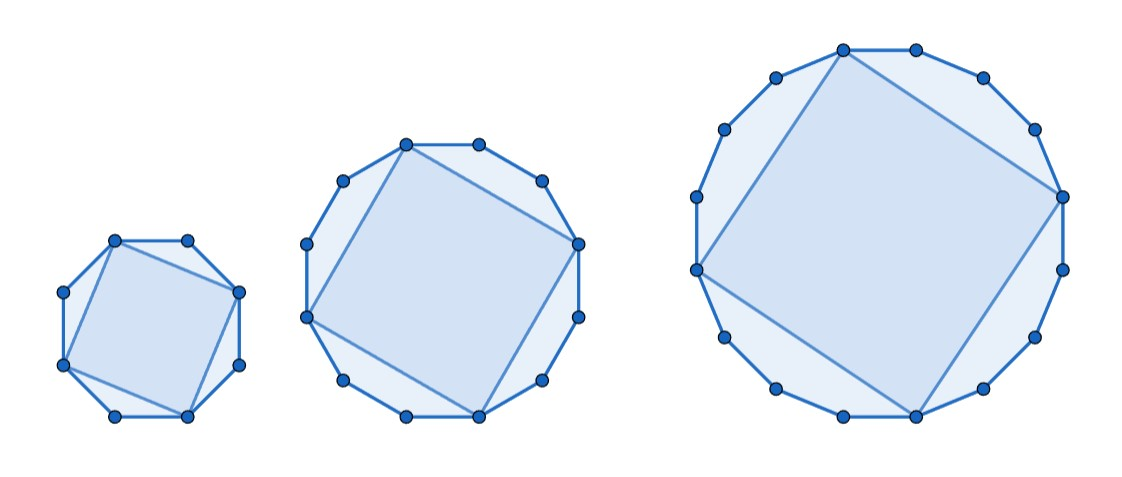
\includegraphics[scale=.75]{images/rq2_1_1.jpg}
	\label{fig:rq2_1_1_img}
	\caption{The figure for finding possible placements for Case 1 of RQ2.}
\end{figure}

Due to the symmetry, as long as vertex B lies on the perimeter of the polygon, the square can be inscribed.
If vertex $B$ lies within the polygon, the square can be fit. We shall find the values of $\theta$ such that the square can be inscribed or fit,
where $\theta = \angle V_{1}OA$.

Firstly, it can be seen that $V_{1}OV_{2} = V_{2}OV_{3} = \cdots = V_{n}OV_{1} = \frac{\ang{360}}{n}$.
Hence, $0 \leq \theta \leq \frac{\ang{360}}{n}$.
Furthermore, we can limit this range to $0 \leq \theta \leq \frac{\ang{180}}{n}$, as when $\theta > \frac{\ang{180}}{n}$, the diagram can be flipped to reduce $\theta$.
We can then try to find $\angle V_{m+1}OB$. To do this, we find the slice of the polygon which contains segment $OB$. We can find the number of triangles that has to be passed through to form $\angle V_{1}OB$. Let this value be $x$. This gives the expression:

\begin{align*}
	 x = \frac{\theta + \ang{90}}{\frac{\ang{360}}{n}}
\end{align*}

Simplifying it,

\begin{align*}
	 x & = \frac{\theta + \ang{90}}{\frac{\ang{360}}{n}}   \\
	 & = \frac{\theta n + \ang{90} n}{\ang{360}} \\
	 & = \frac{\theta n}{\ang{360}} + \frac{n}{4}
\end{align*}

Plugging in the range for $\theta$,

\begin{align*}
	\frac{n}{4} \leq \frac{\theta n}{\ang{360}} + \frac{n}{4} \leq \frac{n}{4} + \frac{1}{2}
\end{align*}

Substituting $n$ for $4m$, 

\begin{align*}
	m \leq x \leq m + \frac{1}{2}
\end{align*}

It can be seen that point $B$ is in triangle $V_{m+1}OV_{m+2}$, and is closer to $V_{m+1}$ than $V_{m+2}$.
We can now check for equality between $OA$ and $OB$, as this would render $ABCD$ as a square.
To do so, the equality $\angle V_{m+1}OB = \angle V_{1}OA$ must be true.

\begin{align*}
	\angle V_{m+1}OB & = \theta + \ang{90} - m\left(\frac{\ang{360}}{n}\right)   \\
	& = \theta
\end{align*}

Hence, a square can always be inscribed.

To find the maximum side length of the square, $OA$ can be maximised. Let $OV_{1} = r$.
Using the Law of Sines,

\begin{figure}[htpb]
	\centering
	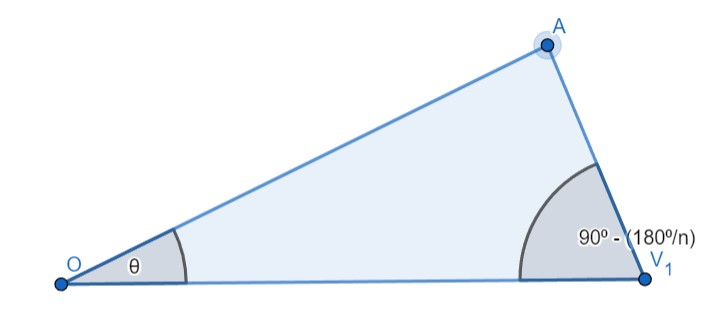
\includegraphics[scale=.75]{images/rq2_1_2.jpg}
	\label{fig:rq2_1_2_img}
	\caption{The triangle formed by point A.}
\end{figure}

\begin{align*}
	\angle AV_{1}O & = \ang{90} - \frac{\ang{180}}{n}     \\
	\frac{OA}{\sin \left(\ang{90} - \frac{\ang{180}}{n}\right)} & = \frac{r}{\sin \left[\ang{180} - \theta - \left(\ang{90} - \frac{\ang{180}}{n}\right)\right]}  \\
	\frac{OA}{\cos \frac{\ang{180}}{n}} & = \frac{r}{\sin \left(\theta + \ang{90} - \frac{\ang{180}}{n}\right)}    \\
	OA & = \frac{r \cos \frac{\ang{180}}{n}}{\cos \left(\frac{\ang{180}}{n} - \theta\right)}
\end{align*}

Notice how the numerator is fixed. To maximise $OA$, $\cos \left(\frac{\ang{180}}{n} - \theta\right)$ needs to be minimised. $\frac{\ang{180}}{n} - \theta$ needs to be maximised, hence $\theta$ must be minimised. This can be done when $\theta = 0$.

The side length of the square can be hence found, $s$, from $r$, and by expressing $r$ from the side length of the entire polygon, $k$, $s$ can be found from $k$ and $n$.

\begin{align*}
	OA & = \frac{r \cos \frac{\ang{180}}{n}}{\cos \left(\frac{\ang{180}}{n}\right)}  \\
	& = r  \\
	s & = OA\sqrt{2} \\
	& = r\sqrt{2} \\
	2r^2 \left(1 - \cos \frac{\ang{360}}{n}\right) & = k^2  \\
	r & = k\sqrt{\frac{1}{2 - 2\cos\frac{\ang{360}}{n}}}  \\
	s & = k\sqrt{\frac{2}{2 - 2\cos\frac{\ang{360}}{n}}}  \\
	& = k\sqrt{\frac{1}{1 - \cos\frac{\ang{360}}{n}}}
\end{align*}

Hence, the side length for a square in such a $n$-gon would be
\begin{equation}
k\sqrt{\frac{1}{1 - \cos\frac{\ang{360}}{n}}}
\end{equation}
where $k$ is the side length of the $n$-gon.

\pagebreak

\subsection{Case 2}
This case deals with the scenario where the number of sides in the $n$-gon is divisible by $2$ but not $4$.

Similar to Case 1 ($4\mid n$), more than one vertex of the square must coincide with the perimeter of the $n$-gon.

Let the square be $ABCD$, and the polygon be $V_{1}V_{2} \cdots V_{n}$. Also, let \(n = 4m + 2\), where $m$ is an integer.

Due to such a polygon being symmetrical both horizontally and vertically, the assumption that the centre of the polygon coincides with the centre of the square can be made. From the earlier observation, it can be assumed that one vertex of the square, $A$, lies on the perimeter of the polygon. Also, due to the polygon being symmetrical both horizontally and vertically, the opposite vertex, $C$, will also lie on the perimeter of the polygon.

\begin{figure}[htpb]
	\centering
	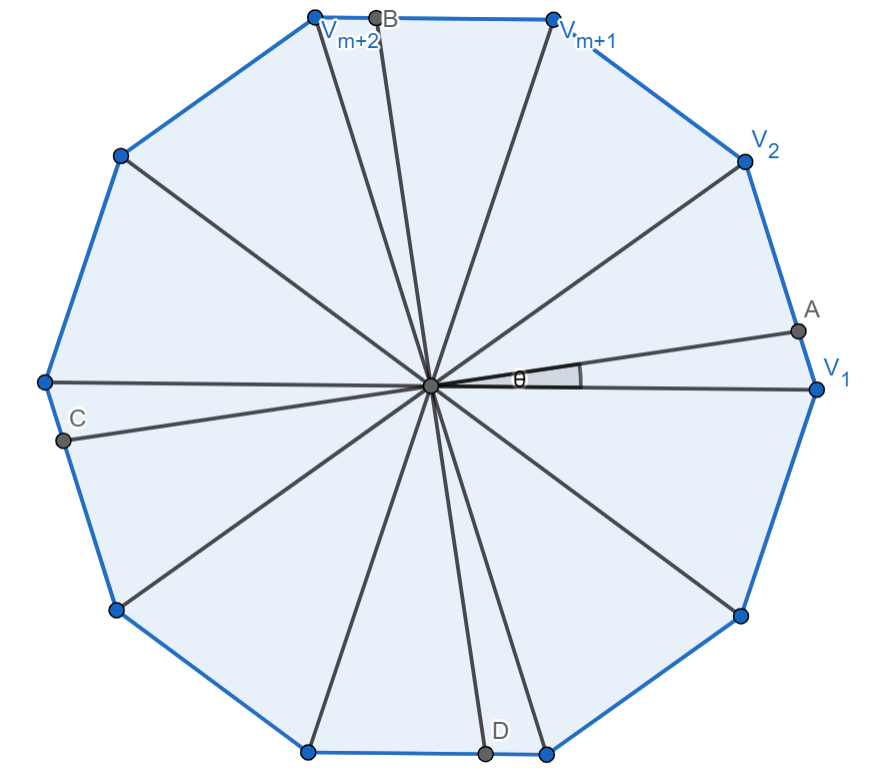
\includegraphics[scale=.75]{images/rq2_2_1.jpg}
	\label{fig:rq2_2_1_img}
	\caption{The figure for finding possible placements for Case 2 of RQ2.}
\end{figure}

Similarly, due to the symmetry, as long as vertex B lies on the perimeter of the polygon, the square can be inscribed.
If vertex $B$ lies within the polygon, the square can be fit. We shall find the values of $\theta$ such that the square can be inscribed or fit,
where $\theta = \angle V_{1}OA$.

We still have the range $0 \leq \theta \leq \frac{\ang{180}}{n}$.
We can then try to find $\angle V_{m+1}OB$. To do this, we can once again find the slice of the polygon which contains segment $OB$. We can find the number of triangles that has to be passed through to form $\angle V_{1}OB$. Let this value be $x$. This gives the expression:

\begin{align*}
	 x = \frac{\theta + \ang{90}}{\frac{\ang{360}}{n}}
\end{align*}

Simplifying it,

\begin{align*}
	 x & = \frac{\theta + \ang{90}}{\frac{\ang{360}}{n}}   \\
	 & = \frac{\theta n + \ang{90} n}{\ang{360}} \\
	 & = \frac{\theta n}{\ang{360}} + \frac{n}{4}
\end{align*}

Plugging in the range for $\theta$,

\begin{align*}
	\frac{n}{4} \leq \frac{\theta n}{\ang{360}} + \frac{n}{4} \leq \frac{n}{4} + \frac{1}{2}
\end{align*}

Substituting $n$ for $4m + 2$, 

\begin{align*}
	m + \frac{1}{2} \leq x \leq m + 1
\end{align*}

It can be seen that point $B$ is in $\triangle V_{m+1}OV_{m+2}$, and is closer to $V_{m+2}$ than $V_{m+1}$.
We can now check for equality between $OA$ and $OB$, as this would render $ABCD$ as a square.
To do so, the equality $\angle V_{m+2}OB = \angle V_{1}OA$ must be true.

\begin{align*}
	\angle V_{m+2}OB & = \left(m+1\right)\left(\frac{\ang{360}}{n}\right) - \ang{90} - \theta \\
	2\theta & = \frac{\ang{360}\left(m+1\right)}{4m+2} - \ang{90}   \\
	2\theta & = \frac{\ang{180}}{4m+2}    \\
	\theta & = \frac{\ang{90}}{n}
\end{align*}

Hence, a square can be inscribed when $\theta = \frac{\ang{90}}{n}$.

To find the side length of the square, we can use the Law of Sines, similar to Case 1. We have:

\begin{align*}
	OA & = \frac{r \cos \frac{\ang{180}}{n}}{\cos \left(\frac{\ang{180}}{n} - \frac{\ang{90}}{n}\right)}  \\
	& = \frac{r \cos \frac{\ang{180}}{n}}{\cos \frac{\ang{90}}{n}}  \\
	s & = OA\sqrt{2} \\
	& = \frac{r \sqrt{2} \cos \frac{\ang{180}}{n}}{\cos \frac{\ang{90}}{n}}  \\
	2r^2 \left(1 - \cos \frac{\ang{360}}{n}\right) & = k^2  \\
	r & = k\sqrt{\frac{1}{2 - 2\cos\frac{\ang{360}}{n}}}  \\
	s & =\frac{k\sqrt{\frac{1}{2 - 2\cos\frac{\ang{360}}{n}}} \sqrt{2} \cos \frac{\ang{180}}{n}}{\cos \frac{\ang{90}}{n}}  \\
	& = \frac{k \cos \frac{\ang{180}}{n}}{\cos \frac{\ang{90}}{n}}\sqrt{\frac{1}{1 - \cos\frac{\ang{360}}{n}}}
\end{align*}

Hence, the expression for the side length of the largest square in such a polygon would be
\begin{equation}
\frac{k \cos \frac{\ang{180}}{n}}{\cos \frac{\ang{90}}{n}}\sqrt{\frac{1}{1 - \cos\frac{\ang{360}}{n}}}
\end{equation}
where $k$ is the side length of the $n$-gon.

\pagebreak

\subsection{Case 3}
Unlike the previous two cases, an $n$-gon with an odd $n$ is not symmetrical horizontally or vertically, hence we cannot make the assumption that the center of the square coincides with the center of the $n$-gon.

Currently, we have no way to assume that the square's vertices lie on the perimeter of the $n$-gon.
This case is still largely a work in progress, and the results obtained so far are inaccurate. However, we have obtained some insights which could aid us in solving this problem.

\begin{itemize}
\item The center of the square cannot coincide with the center of the $n$-gon.
\item One side of the square must be parallel to one side of the $n$-gon.
\end{itemize}

The first of these insights has a simple proof: there are no two parallel lines of symmetry for such a regular polygon, hence if the center of the square were to coincide with the center of the polygon, at least two vertices of the square would not lie on the perimeter of the polygon.

The second of these insights will be explained in further detail in RQ3, below. For now, we shall take it that this statement is true. We can hence calculate the side length using a similar concept to the previous two cases. Furthermore, we also have to account for when $\theta$ lies on the left of the triangle instead of the right.

\begin{figure}[htpb]
	\centering
	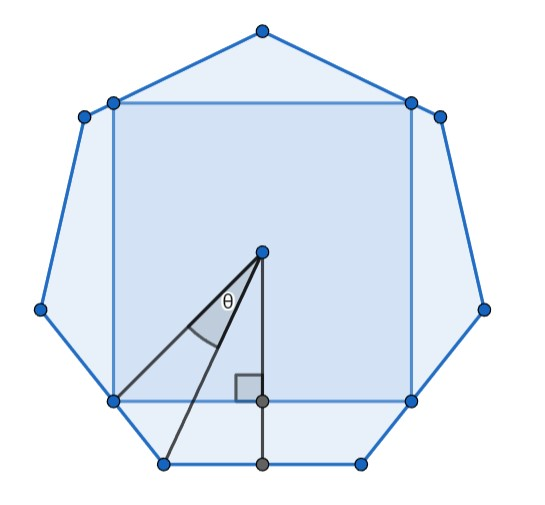
\includegraphics[scale=.75]{images/rq2_3.jpg}
	\label{fig:rq2_3_img}
	\caption{The construction for case 3 of RQ2.}
\end{figure}

\begin{align*}
  \theta & = \min\left[\ang{45} - \frac{\ang{360}}{n}\left\lfloor \frac{\ang{45}}{\frac{\ang{360}}{n}} \right\rfloor, \frac{\ang{360}}{n} - \left(\ang{45} - \frac{\ang{360}}{n}\left\lfloor \frac{\ang{45}}{\frac{\ang{360}}{n}} \rfloor\right)\right]     \\
  & = \min\left[\ang{45} - \frac{\ang{360}}{n}\left\lfloor \frac{n}{8} \right\rfloor, \frac{\ang{360}}{n} - \left(\ang{45} - \frac{\ang{360}}{n}\left\lfloor \frac{n}{8} \rfloor\right)\right]     \\
\end{align*}

\begin{align*}
	OA & = \frac{r \cos \frac{\ang{180}}{n}}{\cos \left\langle\frac{\ang{180}}{n} - \left{\min\left[\ang{45} - \frac{\ang{360}}{n}\left\lfloor \frac{n}{8} \right\rfloor, \frac{\ang{360}}{n} - \left(\ang{45} - \frac{\ang{360}}{n}\left\lfloor \frac{n}{8} \rfloor\right)\right]\right}\right\rangle}  \\
	s & = OA\sqrt{2} \\
	& = \frac{r \sqrt{2} \cos \frac{\ang{180}}{n}}{\cos \left\langle\frac{\ang{180}}{n} - \left{\min\left[\ang{45} - \frac{\ang{360}}{n}\left\lfloor \frac{n}{8} \right\rfloor, \frac{\ang{360}}{n} - \left(\ang{45} - \frac{\ang{360}}{n}\left\lfloor \frac{n}{8} \rfloor\right)\right]\right}\right\rangle}  \\
\end{align*}

\begin{align*}
	k^2 & = 2r^2 \left(1 - \cos \frac{\ang{360}}{n}\right)  \\
	r & = k\sqrt{\frac{1}{2 - 2\cos\frac{\ang{360}}{n}}}  \\
	s & = \frac{k\sqrt{\frac{1}{2 - 2\cos\frac{\ang{360}}{n}}} \sqrt{2} \cos \frac{\ang{180}}{n}}{\cos \left\langle\frac{\ang{180}}{n} - \left{\min\left[\ang{45} - \frac{\ang{360}}{n}\left\lfloor \frac{n}{8} \right\rfloor, \frac{\ang{360}}{n} - \left(\ang{45} - \frac{\ang{360}}{n}\left\lfloor \frac{n}{8} \rfloor\right)\right]\right}\right\rangle}  \\
	& = \frac{k \cos \frac{\ang{180}}{n}}{\cos \left(\frac{\ang{180}}{n} - \left{\min\left[\ang{45} - \frac{\ang{360}}{n}\left\lfloor \frac{n}{8} \right\rfloor, \frac{\ang{360}}{n} - \left(\ang{45} - \frac{\ang{360}}{n}\left\lfloor \frac{n}{8} \rfloor\right)\right]\right}\right)} \sqrt{\frac{1}{1 - \cos\frac{\ang{360}}{n}}} \\
\end{align*}

\section{Research Question 3}
RQ3 aims to find the largest square that can be inscribed in a convex polygon, given the side lengths of the polygon.
We were unable to find this due to the vagueness of the question. However, we are still able to prove certain things.

\subsection{Proof that a square can always be inscribed}
We have proved that a square can always be inscribed in a convex polygon.

We first construct an arbitary line $A_{1}A_{2}$. Then, at every vertex, we draw a line parallel to $A_{1}A_{2}$.

\begin{figure}[htpb]
	\centering
	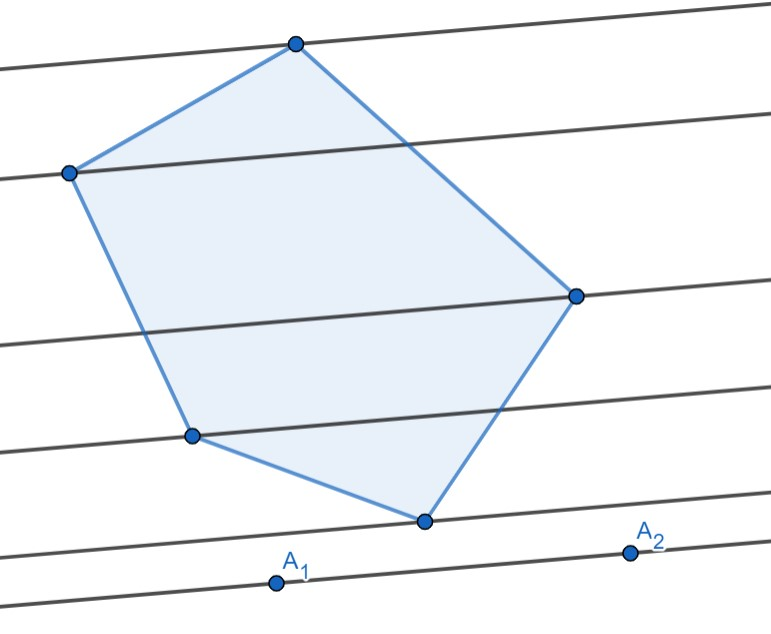
\includegraphics[scale=.75]{images/rq3_1_1.jpg}
	\label{fig:rq3_1_1_img}
	\caption{The construction for RQ3.}
\end{figure}

We can get the midpoint of the newly formed line segments in the polygon, and connect them together. We shall call the line segments that connect the midpoints together the \textbf{first group} of line segments, as shown in Figure 6.

\begin{figure}[htpb]
	\centering
	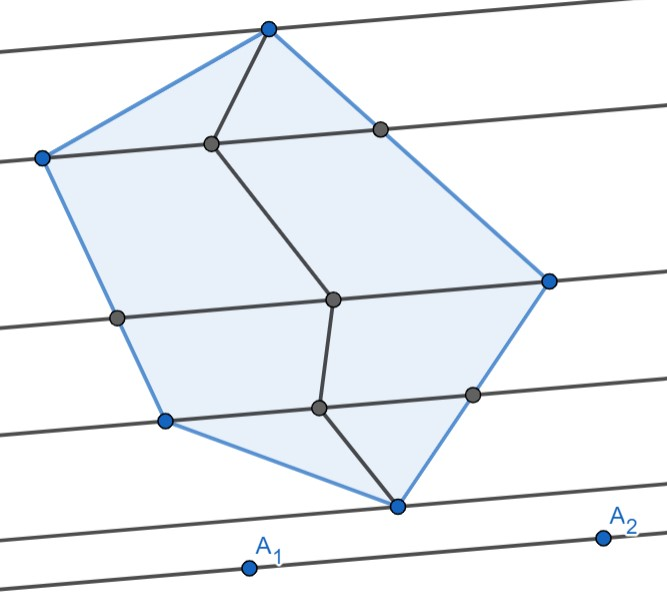
\includegraphics[scale=.75]{images/rq3_1_2.jpg}
	\label{fig:rq3_1_2_img}
	\caption{The construction of the first group of line segments.}
\end{figure}

Now, we draw a line perpendicular to $A_{1}A_{2}$ at every vertex, get the midpoint of the newly formed line segments, and connect them together. We shall call the line segments that connect the midpoints together the \textbf{second group} of line segments, as shown in Figure 7.

\begin{figure}[htpb]
	\centering
	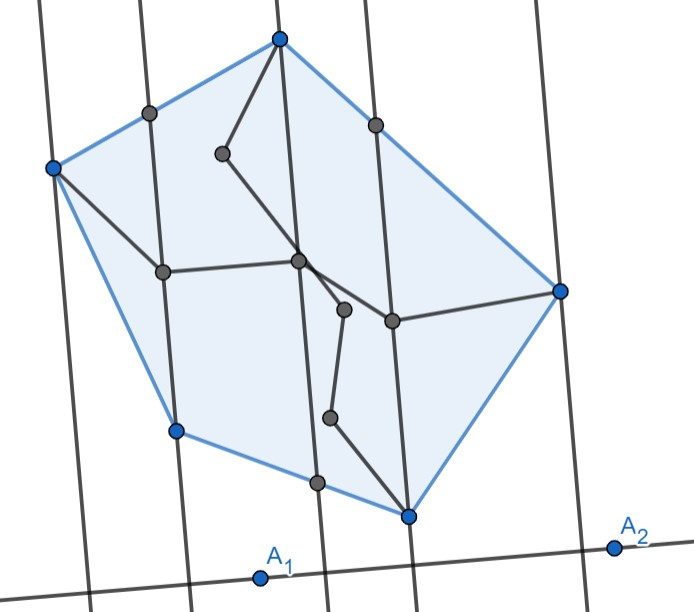
\includegraphics[scale=.75]{images/rq3_1_3.jpg}
	\label{fig:rq3_1_3_img}
	\caption{The construction of the second group of line segments.}
\end{figure}

Notice how the two groups intersect at one point. Let this point be $O$. We draw a line parallel to $A_{1}A_{2}$ at point $O$.
We then draw another line perpendicular to $A_{1}A_{2}$ at $O$. Notice how the four intersections between these two lines and the perimeter of the polygon form a rhombus. Let this rhombus be $ABCD$. This is illustrated in Figure 8.

\begin{figure}[htpb]
	\centering
	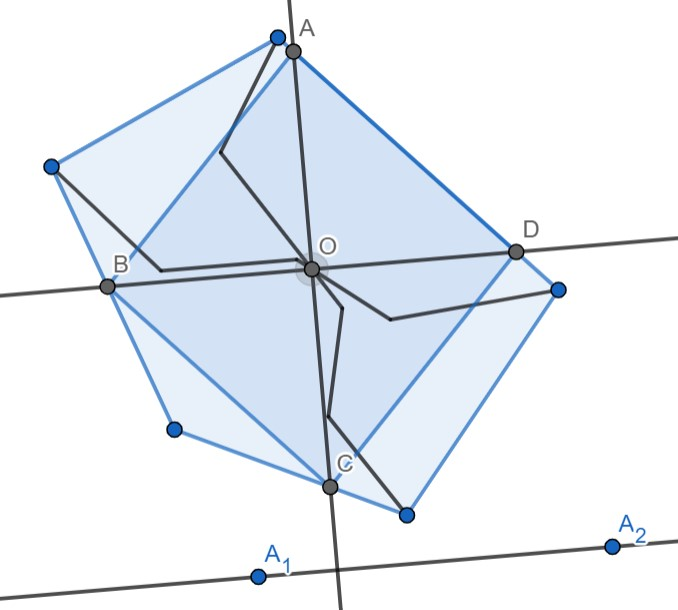
\includegraphics[scale=.75]{images/rq3_1_4.jpg}
	\label{fig:rq3_1_4_img}
	\caption{The construction of the rhombus.}
\end{figure}

Do note that this rhombus need not be a square. However, using the Intermediate Value Theorem, we can show that if $A_{1}A_{2}$ is rotated clockwise enough, the rhombus will be a square.

\subsection{Proof for Case 3 of RQ2}
In RQ2, we mentioned that one side of the square had to be parallel to one side of the polygon. This can be proven using the concept presented above:
We know that a construction where one side of the square is parallel to one side of the polygon exists. In this case, $A_{1}A_{2}$ is $\ang{45}$ away from the base of the polygon. It can be seen that by making the angle between $A_{1}A_{2}$ and the base of the polygon smaller, 2 of the angles of the rhombus will increase, and 2 will decrease and vice versa.
Hence, the only occurrence where the rhombus is a square and all four angles of the rhombus are equal is when $A_{1}A_{2}$ is $\ang{45}$ away from the base of the polygon.

\section{Conclusion and Further Work}
All in all, we were able to solve most of our research questions. However, as RQ3 was very vague, it was more difficult than the others, leading to us being unable to complete it. One potential continuation of the project is that, besides completing RQ3, we can also address concave polygons, or even curves. Such a continuation would be able to address things such as the inscribed square problem. Other possible extension methods would be to extend this problem to 3D space, for example, by fitting cubes into prisms with different $n$-gons as bases.   

\printbibliography
\end{document}
